\documentclass[letterpaper]{article}
\usepackage[spanish,es-tabla]{babel}
\usepackage{indentfirst}
\usepackage{float}
\usepackage[utf8]{inputenc}
\usepackage{graphicx}
\usepackage{hyperref}
\title{Evaluación DSP}
\author{Saez, Lautaro Andres}

\begin{document}

    \section{Ejercicio 2}

    En este inciso se analizara el caso de que una señal es periodica y continua. Se utilizara la siguiente señal: 

    \begin{equation}
        \label{eq.punto2}
        x_c(t) = sin( 200 \pi t )
    \end{equation}

    \subsection*{Inciso a)}

    En este inciso se calcula la CTFS de eq.\ref{eq.punto2}. Se sabe con anterioridad que la CTFS de una señal
    esta definida:
    
    \begin{equation}
        x(t)= \sum_{k=-\infty}^{\infty} a_k e^{j\omega_0 kt}
    \end{equation}

    \begin{equation}
        a_k = \frac{1}{T} \int_{-T/2}^{T/2} x(t)e^{-j\omega_0 kt}
    \end{equation}

    Aplicando la formula de Euler a la eq.\ref{eq.punto2} se obtiene 

    \begin{equation}
        x_c(t)=\frac{1}{2j}( e^{j200\pi t} - e^{-j200 \pi t})
    \end{equation}

    Es posible apreciar que los coeficientes de la serie son: 

    \begin{equation}
        c_1 = \frac{1}{2j} \hspace*{.1cm} \land \hspace*{.1cm} c_{-1}=-\frac{1}{2j}
    \end{equation}

    \subsection*{Inciso b)}

    En este inciso se muestrea la señal a una frecuencia adecuada, y luego se le calcula de DFT.

    Aplicando el teorema del muestreo, se debe elegir una frecuencia mayor a $2F_N$, siendo 
    en este caso $F_N=100Hz$, por ello se utilizara $F_s=400Hz$. Con dicha frecuencia se obtiene 

    \begin{equation}
        x[n]=x(n/F_s) \rightarrow x[n]= sin\left( \frac{\pi}{2} n\right)
    \end{equation}

    Cuyo periodo fundamental ($N_0$) es $4$.

    Aplicando la eq.\ref{eq.DFT}

    \begin{equation}
        X[k]= \sum_{n=0}^{3} sin\left( \frac{\pi}{2} n\right) e^{-j\frac{\pi}{2} nk}
    \end{equation}

    Calculando los valores de $x[n]$ para $n\in {1, 2, 3 ,4}$

    \begin{table}[H]
        \centering
        \begin{tabular}{|c|c|}
            \hline $n$ & $sin(\pi n/2)$ \\ 
            \hline $0$ & $0$ \\
            \hline $1$ & $1$ \\
            \hline $2$ & $0$ \\
            \hline $3$ & $-1$ \\
            \hline
        \end{tabular}
        \caption{Valores de la señal muestreada en 1 periodo.}
    \end{table}

    Reemplazando en la ecuacion anterior, se obtiene 

    \begin{equation}
        X[k]= e^{-j\frac{\pi}{2}k} - e^{-j\frac{ 3 \pi}{2}k}
    \end{equation}

    Es posible expresar a $e^{-j\frac{ 3 \pi}{2}k}$ como $e^{-j \frac{\pi }{2}k}e^{-j\pi k}$, aplicando la identidad de Euler 
    $e^{-j \pi k}= (-1)^k$. 

    \begin{equation}
        X[k]= [ 1 + (-1)^{k+1} ] e^{ -j \frac{\pi }{2} k }
    \end{equation}

    \begin{table}[H]
        \centering
        \begin{tabular}{|c|c|}
            \hline $k$ & $X[k]$ \\
            \hline $0$ & $0$ \\
            \hline $1$ & $-2j$ \\
            \hline $2$ & $0$ \\
            \hline $3$ & $2j$ \\
            \hline
        \end{tabular}
        \caption{Valores de $X[k]$.}
        \label{tab.xk}
    \end{table}

    \subsection*{Inciso c)}

    En este inciso se analiza la relacion entre la CTFS y DFT, y si es posible calcular la CTFS a partir de la CTFS sin error.

    Al dividir los coeficientes $X[k]$ (Tab.\ref{tab.xk}) por el el numero de muestras $N$, el resultado son los coeficientes 
    $c_k$. Luego se puede establecer a priopi la relacion 
    
    \begin{equation}
        c_k = \frac{X[k]}{N}
    \end{equation}

    Para la ecuacion anterior se aplica el conocimiento que $X[k]$ es periodica, y por lo tanto $X[-1]=X[3]$.

    Cabe mencionar que si la señal se encuentra bien muestreada (cumple el teorema de muestreo) y en el caso de que la señal sea de banda limitada (tenga un número finito de 
    armónicos) como en este caso, se puede obtener de manera exacta la aproximación sin error. Pero en el caso de tener una señal que no sea de banda limitada (como el caso de un cajón) se tendria un error debido 
    a que no es posible cumputacionalmente realizar el cálculo con infinitos valores.


    \subsection*{Inciso d)}

    En este inciso se genera una cantidad enteras de periodos de la señal muestreada,
    para luego calcular la DFT y verificar las conclusiones obtenidas en el inciso anterior.

    \begin{figure}[H]
        \centering
        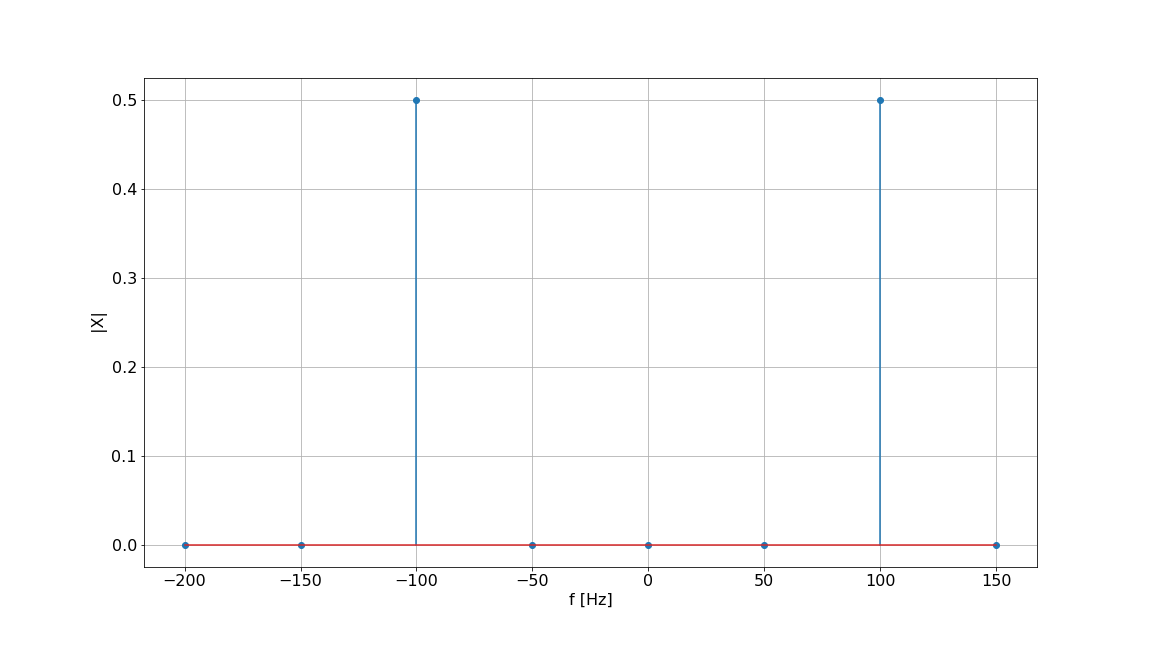
\includegraphics[width=\textwidth]{Img/punto_2_d.png}
        \caption{CTFS obtenida mediante el algoritmo de FFT para N=4.}
        \label{fig.2d}
    \end{figure}
    Es posible obervar en la Fig.\ref{fig.2d} se cumple la ide previa concebida em el inciso anterior.
    
    \subsection*{Inciso e)}

    En este inciso se agrega 1 muestras mas, y se analiza lo que sucede con la DFT.

    \begin{figure}[H]
        \centering
        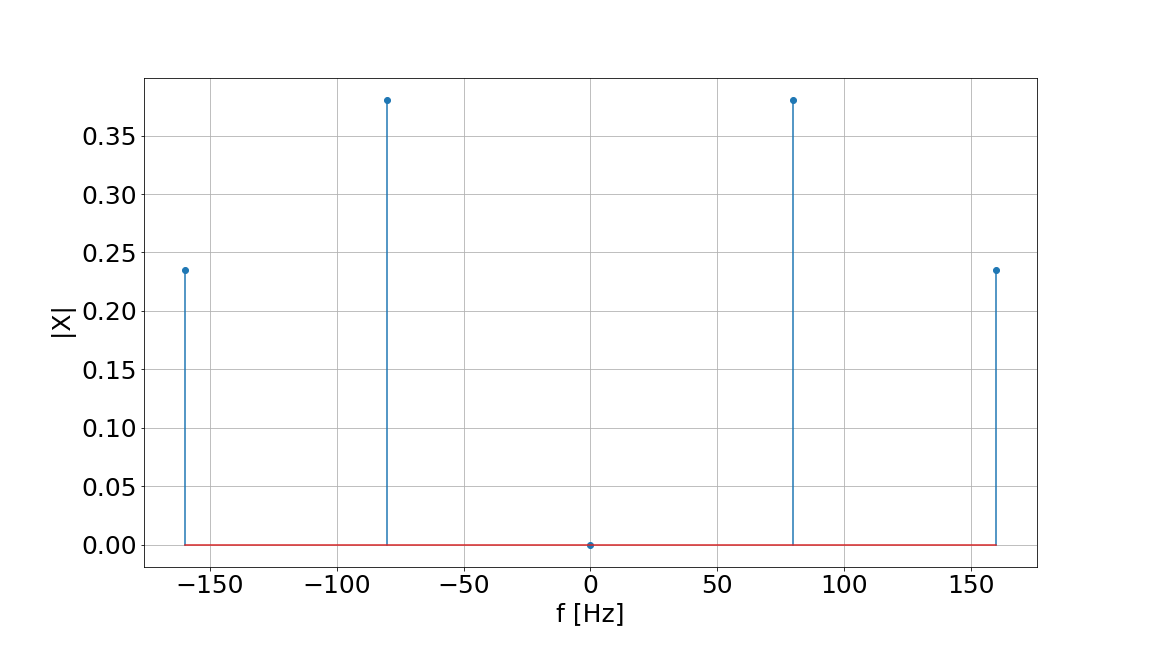
\includegraphics[width=\textwidth]{Img/punto_2_e.png}
        \caption{CTFS obtenida para N=5}
        \label{fig.2e}
    \end{figure}

    Al añadir una muestra mas a la señal ingresada, debido a como se implementa el algoritmo, la señal se ve modificada y su 
    extension periodicica es diferente, similar a lo que sucedio en el inciso 1-e, por lo que se observa en fig.\ref{fig.2e} aparecen 
    valores de frecuencia que no son los esperados;
    este error debido a como se implementa la DFT, ya que el algoritmo ve una señál de periodo 5, en este caso, la cual no 
    representa la señal real, y por lo tanto el espectro no coincide con el de la señál original.


    \subsection*{Inciso f)}

    En este inciso se establecen las condiciones para poder obtener de forma exacta la 
    CTFS a partir de la DFT.

    Para obtener la CTFS usando la FFT, es necesario realizar un buen muestreio de la señal, 
    para obtener la señal muestrada. A dicha señal se apalica la FFT con el número correspondiente
    de puntos (se debe cumplir que el número de puntos tomados sea mayor o igual al número minimo de puntos que representa un periodo de la señal). 
    Posteriormente se normaliza con el valor de puntos 
    y de esa manera se obtiene la CTFS aproximada aplicando la FFT.

    Por otro lado, para que la representación sea exacta se deben cumplir las siguientes condiciones:
    \begin{enumerate}
        \item La señal original debe ser de banda limitada.
        \item Se debe muestrear respetando el teorema de muestreo $F_s\geq 2F_N$
        \item El número de puntos que se usan en la FFT debe ser un multiplo del numero de muestras que representan un periodo ($N\geq L$)
    \end{enumerate}

    \subsection*{Inciso g)}

    En este inciso se comprueba de forma practica las conclusiones obtenidas en 
    el inciso anterior, las siguientes señales 
    
    \begin{enumerate}
        \item $x_1(t)= 4 sen( 2\pi 1000 t ) + 3sen( 2\pi 2000 t ) + 2sen( 2\pi 3000 t )$
        \item $ x_2(t)= \sum_{l=-\infty}^{\infty} \mu( t - 10l - 2  )\mu( 2 + 10l - t )$
    \end{enumerate}

    \subsubsection*{1}

    Para poder comparar y verificar el correcto funcionamiento del algoritmo de FFT
    se buscara la CTFS de forma teorica, para ello se aplica la formula de Euler
    
    \begin{equation}
        x_1(t) = \frac{1}{2j} ( 4e^{j2000 \pi t} - 4e^{-j2000 \pi t}  +3e^{j4000 \pi t} - 3e^{-j4000 \pi t} +2e^{j6000 \pi t} - 2e^{-j6000 \pi t} )
    \end{equation}

    

    Por lo se obtienen los coeficietes de la serie de forma sencilla tab.\ref{tab.2gi}.

    \begin{table}[H]
        \centering
        \begin{tabular}{|c|c|}
            \hline $k$ & $c_k$ \\ 
            \hline $-3$ & $j$ \\
            \hline $-2$ & $3j/2$ \\ 
            \hline $-1$ & $2j$ \\ 
            \hline $0$ & $0$ \\ 
            \hline $1$ & $-2j$ \\ 
            \hline $2$ & $-3j/2$ \\ 
            \hline $3$ & $-j$ \\ 
            \hline
        \end{tabular}
        \caption{Coeficientes $c_k$.}
        \label{tab.2gi}
    \end{table}

    Para calcular la DFT se debe seleccionar una frecuencia de muestreo, debido a que la frecuencia maxima de la señál es de $3000Hz$ se
    toma $F_s = 9000 muestras / seg$.

    \begin{figure}[H]
        \centering
        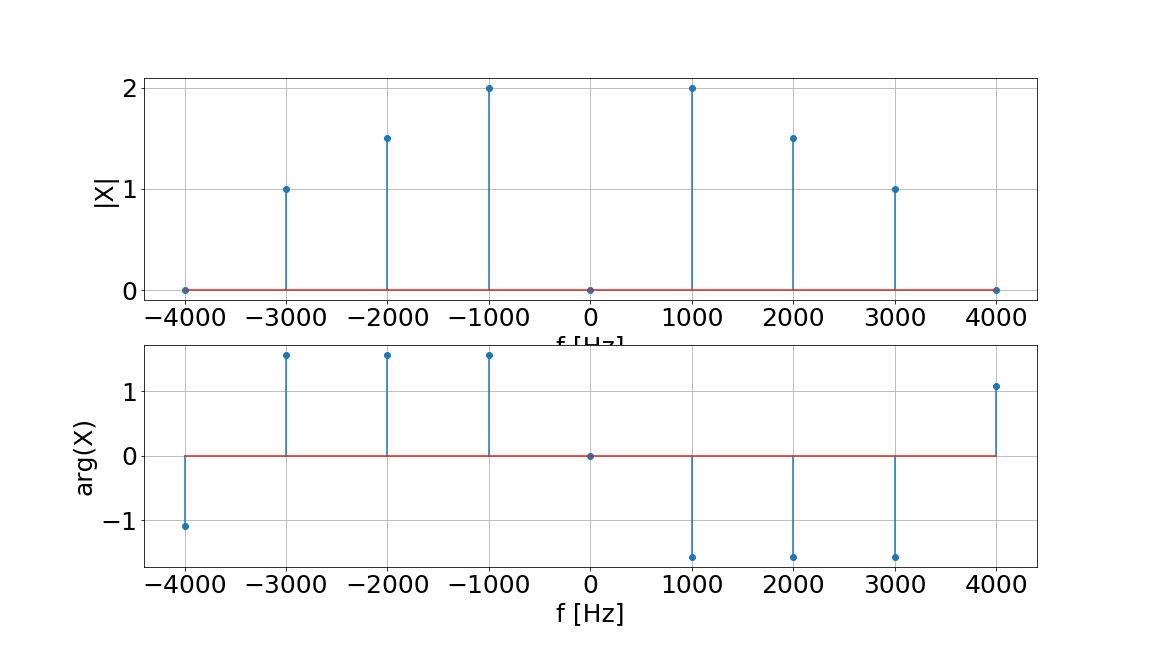
\includegraphics[width=\textwidth]{Img/punto_2_g_1.png}
        \caption{CTFS de $x_1(t)$ obtenida con el algoritmo de FFT.}
        \label{fig.2gi}
    \end{figure}
    
    \subsubsection*{2}

    Dicha ecuacion describe un tren de pulsos de ancho $4$ y periodo $10$, al calcular los coeficientes de la CTFS se obtienen
    infinitos valores cuya envolvente es una $sinc$, debido a que la señal no es de banda limitada no sera posible recuperara su espectro 
    de forma completa. 

    \begin{equation}
        a_k = \frac{4}{10} sinc \left( \frac{2}{4}k \right)
    \end{equation}

    Debido a que no sera posible recuperar el espectro de la señal original, pero si aproximarlo, se toma $F_s=5 muestras/seg$, para
    obtener una aproximacion aceptable, en caso el periodo de la señal muestreada sera de $50 muestras$.

    \begin{figure}[H]
        \centering
        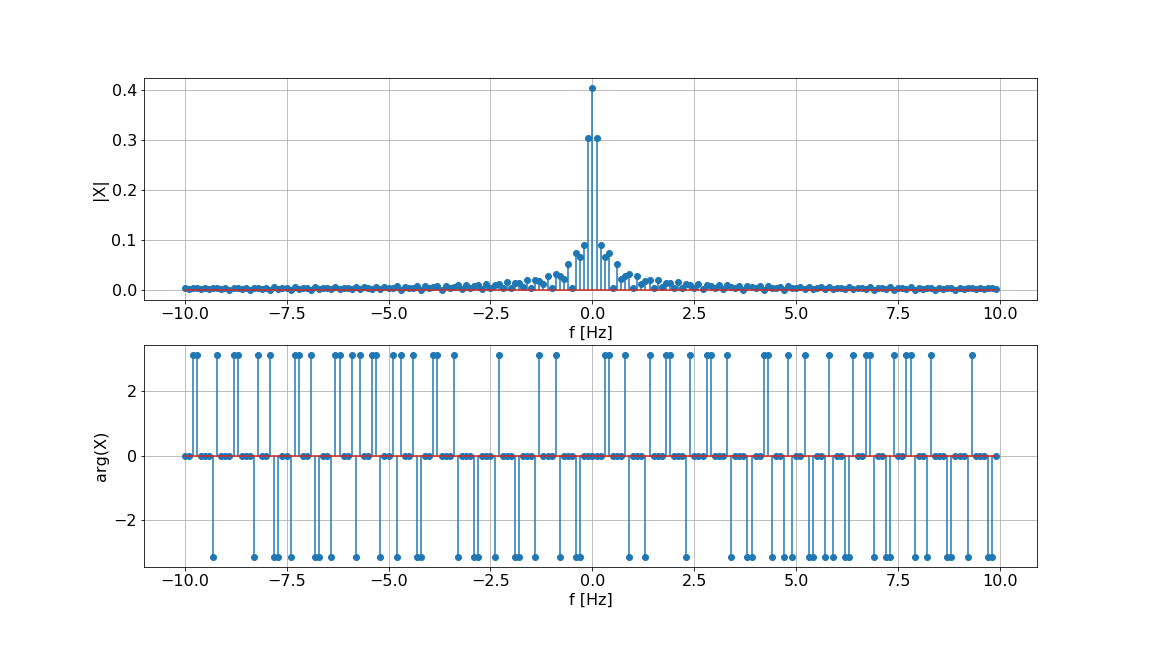
\includegraphics[width=\textwidth]{Img/punto_2_g_2.png}
        \caption{CTFS de $x_2(t)$ con $F_2=5 muestras/s$ y $N=50$ y la envolvente.}
        \label{fig.2gii}
    \end{figure}

    En la fig.\ref{fig.2gii} se observa como el valores de los coeficientes obtenidos difiere con los valores reales,
    aunque se puede concluir que dicha aproximacion es util para estimar el espectro, de forma adicional se incluye un \href{https://drive.google.com/open?id=10pVC59n6z_zfX6Qlm4w96l_1q3lnr2g6}{\underline{video}}
    donde es posible observar como al variar $F_s$ los coeficientes de la CTFS se ajustan cada vez mejor a los valores de la envolvente, cabe destacar que nunca se podra obtener de forma 
    exacta la CTFS, pero si es posible lograr una muy buena aproximacion.


\end{document}